\chapter{DESENVOLVIMENTO}

\section{Apresentação do Sistema}

O sistema desenvolvido, denominado \textbf{NaraPsi}, consiste em uma plataforma digital voltada ao gerenciamento seguro de informações clínicas utilizadas por profissionais da área da psicologia. O objetivo principal da plataforma é centralizar o armazenamento e a organização de documentos terapêuticos, tais como anamneses, registros de sessões, laudos, pareceres psicológicos, encaminhamentos e demais documentos relacionados ao acompanhamento clínico de pacientes.

Tradicionalmente, esses documentos são elaborados e armazenados utilizando ferramentas genéricas de edição de texto e serviços de armazenamento em nuvem, o que frequentemente resulta em fragmentação das informações, dificuldades de organização e riscos relacionados à segurança de dados sensíveis. Nesse contexto, o NaraPsi foi projetado para oferecer um ambiente digital especializado para o gerenciamento estruturado de informações clínicas.

O sistema foi concebido considerando os princípios fundamentais de segurança da informação — confidencialidade, integridade e disponibilidade — além da conformidade com a Lei Geral de Proteção de Dados (Lei nº 13.709/2018). Para isso, foram implementados mecanismos de autenticação segura, controle de acesso baseado em perfis, criptografia de dados sensíveis e registro auditável de operações realizadas na plataforma.

Um dos diferenciais da solução proposta é a integração de mecanismos de inteligência artificial aplicados ao Processamento de Linguagem Natural (Natural Language Processing – NLP). Por meio da utilização de modelos de linguagem de grande escala (Large Language Models – LLMs), o sistema é capaz de auxiliar o profissional na geração automatizada de documentos clínicos e na análise contextual de informações registradas ao longo do acompanhamento terapêutico.

A plataforma foi projetada seguindo o paradigma de aplicações web modernas, com arquitetura cliente-servidor e interface acessível por navegadores em diferentes dispositivos. Dessa forma, busca-se garantir não apenas segurança e confiabilidade no tratamento dos dados, mas também usabilidade e eficiência no fluxo de trabalho dos profissionais de saúde mental.

\section{Metodologia de Desenvolvimento}

O desenvolvimento do sistema foi conduzido utilizando a metodologia ágil \textit{Scrum}, amplamente adotada em projetos de engenharia de software que demandam flexibilidade, adaptação contínua e entregas incrementais.

O Scrum estrutura o processo de desenvolvimento em ciclos iterativos denominados \textit{sprints}, nos quais funcionalidades específicas são planejadas, implementadas, testadas e avaliadas. Essa abordagem permite a evolução progressiva do sistema, com validação constante das funcionalidades desenvolvidas.

Cada sprint teve duração média de duas semanas e envolveu atividades de planejamento, implementação, testes e revisão das funcionalidades desenvolvidas. Ao final de cada ciclo, foi realizada uma análise do progresso obtido e da adequação das funcionalidades implementadas em relação aos requisitos do sistema.

A utilização dessa metodologia foi particularmente relevante considerando a natureza exploratória de algumas funcionalidades do projeto, especialmente aquelas relacionadas à integração de modelos de inteligência artificial e geração automatizada de documentos clínicos.

\subsection{Etapas do Processo}

\textbf{Levantamento de Requisitos} Inicialmente foi realizado um processo de levantamento de requisitos junto a profissionais da área da psicologia, com o objetivo de compreender os fluxos de trabalho existentes, os principais documentos utilizados na prática clínica e as dificuldades enfrentadas na gestão de informações de pacientes.

\textbf{Projeto da Arquitetura} A partir dos requisitos levantados, foi definida a arquitetura do sistema, incluindo as tecnologias utilizadas, a estrutura do banco de dados e os mecanismos de segurança necessários para garantir a proteção das informações sensíveis.

\textbf{Implementação} Durante as sprints de desenvolvimento, as funcionalidades foram implementadas de forma incremental, priorizando inicialmente os componentes responsáveis por autenticação, controle de acesso, gerenciamento de pacientes e armazenamento de documentos.

Posteriormente foram integradas funcionalidades mais avançadas, como geração automatizada de documentos utilizando modelos de linguagem e integração com sistemas de assinatura digital.

\textbf{Testes} Cada funcionalidade implementada passou por ciclos de testes unitários e testes de integração, com o objetivo de garantir a correta execução das operações e a integridade das informações manipuladas pelo sistema.

\textbf{Validação} As funcionalidades implementadas foram avaliadas considerando critérios de segurança, usabilidade e desempenho, buscando assegurar que o sistema atendesse às necessidades práticas dos profissionais que utilizarão a plataforma.

\subsection{Histórias de Usuários}

A identificação das histórias de usuários foi realizada a partir de entrevistas e conversas com psicólogos atuantes na prática clínica, com o objetivo de compreender os fluxos de trabalho atuais, os principais documentos utilizados, as dificuldades enfrentadas na gestão documental e as expectativas em relação ao uso de tecnologias como a inteligência artificial.

De acordo com os profissionais consultados, os documentos mais comumente gerados são: anamnese, relatos psicológicos, parecer psicológico, laudos, atestados, encaminhamentos e declarações. Todos esses documentos requerem assinatura do psicólogo para garantir sua validade legal, e no caso da anamnese, é também exigida a assinatura do paciente. Atualmente, os profissionais utilizam ferramentas genéricas, como Microsoft Word ou Google Docs, para redigir esses documentos, sendo que o armazenamento é feito de maneira descentralizada — em computadores pessoais, serviços de nuvem como Google Drive e OneDrive ou até mesmo em formato físico. Essa falta de padronização representa um risco à segurança e confidencialidade dos dados dos pacientes.

Durante as entrevistas, os psicólogos também relataram grande interesse no uso de ferramentas baseadas em inteligência artificial (IA), especialmente para a geração automatizada de documentos padronizados, como laudos, pareceres e encaminhamentos. Segundo os profissionais, a IA poderia ainda facilitar o acesso a informações específicas sobre os pacientes, como medicamentos em uso, sintomas relatados, queixas recorrentes, composição familiar e rotina diária. Atualmente, a obtenção dessas informações exige a leitura manual de todos os relatos de sessões anteriores, o que consome tempo e dificulta a prática clínica.

\subsection{Prototipação}
Averiguar necessidade para cada projeto.

\section{Requisitos do Sistema}

\subsection{Requisitos Funcionais}

\begin{table}[H]
\centering
\caption{Requisitos Funcionais do Sistema}
\begin{tabular}{@{}lp{13cm}@{}}
\toprule
\rowcolor[HTML]{EFEFEF} 
\textbf{Nº} & \textbf{Descrição do Requisito Funcional} \\ \midrule
RF1.  & O sistema deve permitir o cadastro de pacientes, contendo informações pessoais, contato e histórico terapêutico. \\
RF2.  & O sistema deve permitir a geração de documentos terapêuticos, incluindo anamnese, relatos psicológicos, pareceres, laudos, atestados, encaminhamentos e declarações. \\
RF3.  & O sistema deve permitir a assinatura digital de documentos pelo psicólogo, com validade jurídica, conforme legislação vigente. \\
RF4.  & O sistema deve possibilitar o armazenamento seguro e centralizado de todos os documentos gerados, vinculando-os aos respectivos pacientes. \\
RF5.  & O sistema deve disponibilizar modelos de documentos personalizáveis pelo profissional, de acordo com sua abordagem terapêutica. \\
RF6.  & O sistema deve permitir a anexação de arquivos externos (como PDFs, imagens ou exames) aos registros do paciente. \\
RF7.  & O sistema deve integrar uma funcionalidade de Inteligência Artificial capaz de gerar documentos automaticamente a partir de dados fornecidos ou relatórios anteriores. \\
RF8.  & O sistema deve permitir consultas automatizadas por meio da IA para extração de informações específicas do histórico do paciente. \\
RF9.  & O sistema deve permitir o gerenciamento de usuários e autenticação por credenciais seguras. \\
RF10. & O sistema deve manter um registro de atividades e alterações realizadas nos documentos e cadastros. \\
\bottomrule
\end{tabular}
\label{tab:req-funcionais}
\end{table}

\subsection{Requisitos Não Funcionais}

\begin{table}[H]
\centering
\caption{Descrição do Requisito Não-Funcional}
\begin{tabular}{@{}lp{13cm}@{}}
\toprule
\rowcolor[HTML]{EFEFEF} 
\textbf{Nº} & \textbf{Descrição do Requisito Não Funcional} \\ \midrule
RNF1.  & O sistema deve garantir a segurança dos dados armazenados, utilizando criptografia para arquivos e comunicações, conforme os princípios da LGPD. \\
RNF2.  & O sistema deve estar em conformidade com as normas de proteção de dados pessoais sensíveis, especialmente os de saúde, conforme a Lei nº 13.709/2018. \\
RNF3.  & O sistema deve oferecer alta disponibilidade e redundância nos dados, para garantir que informações não sejam perdidas em caso de falha. \\
RNF4.  & O sistema deve possuir uma interface web responsiva e intuitiva, acessível em diferentes dispositivos (computadores, tablets e celulares). \\
RNF5.  & O sistema deve ser compatível com navegadores modernos (Chrome, Firefox, Edge, Safari) e não exigir instalações adicionais no dispositivo do usuário. \\
RNF6.  & O tempo de resposta para geração de documentos automatizados via IA deve ser inferior a 30 segundos em condições normais de operação. \\
RNF7.  & O sistema deve utilizar protocolos seguros (HTTPS/TLS) para toda comunicação entre cliente e servidor. \\
RNF8.  & A plataforma deverá ser desenvolvida com arquitetura modular para facilitar a manutenção e futura escalabilidade. \\
RNF9.  & A plataforma deve integrar com a API de assinatura digital do ClickSign. \\
RNF10. & O sistema deve armazenar os documentos em formato PDF/A, garantindo sua legibilidade e validade jurídica a longo prazo. \\
\bottomrule
\end{tabular}
\label{tab:req-nao-funcionais}
\end{table}

\section{Regras de Negócio}

Esta seção apresenta as regras de negócio definidas para o sistema, que orientam o comportamento da aplicação no que diz respeito à segurança da informação, integridade dos dados, controle de acesso e conformidade legal, especialmente considerando os requisitos próprios da atuação psicológica e os preceitos estabelecidos pela Lei Geral de Proteção de Dados (LGPD).

\begin{table}[H]
\centering
\caption{Regras de Negócio}
\begin{tabular}{@{}lp{13cm}@{}}
\toprule
\rowcolor[HTML]{EFEFEF} 
\textbf{Código} & \textbf{Descrição da Regra de Negócio} \\ \midrule
RN01 & Psicólogos autenticados devem ter acesso apenas aos dados dos pacientes por eles cadastrados ou vinculados. \\
RN02 & Uma vez assinado, o documento permanecerá disponível permanentemente para leitura por todas as partes que o assinaram. \\
RN03 & Todos os documentos possuem dois estados: "Em elaboração" e "Finalizado". Documentos "Em elaboração" podem ser editados; documentos "Finalizado" são imutáveis. \\
RN04 & Para que um documento passe para o estado "Finalizado", é obrigatória a presença de ao menos uma assinatura digital válida. \\
RN05 & Apenas psicólogos autenticados podem visualizar, editar, criar ou assinar documentos vinculados aos seus pacientes. \\
RN06 & Toda ação que resulte em modificação na base de dados deve ser registrada em uma tabela de logs, identificando o autor e a ação realizada. \\
RN07 & Documentos assinados não poderão ser excluídos definitivamente. Qualquer exclusão será apenas lógica e registrada com data, hora e autor da ação. Documentos excluídos com mais de 5 anos de sua criação serão excluídos em definitivo da plataforma. \\
RN08 & Todos os dados dos pacientes e seus documentos devem ser criptografados tanto em repouso quanto em trânsito, conforme a Lei nº 13.709/2018 (LGPD). \\
RN09 & A IA pode sugerir trechos ou modelos de documentos, mas a responsabilidade pela validação e assinatura é exclusiva do psicólogo. \\
RN10 & O sistema deve exportar documentos em formato PDF/A, que garante validade jurídica e arquivamento eletrônico de longo prazo. \\
RN11 & Psicólogos não devem ter acesso a dados de pacientes vinculados a outros profissionais, respeitando o sigilo terapêutico. \\
RN12 & A geração de conteúdo automatizado pela IA deve considerar apenas os dados registrados previamente nos atendimentos e relatórios. \\
RN13 & Deve ser possível o download dos documentos em formato PDF/A apenas pelo usuário que originalmente o criou. \\
RN14 & Um usuário poderá possuir um ou mais perfis de acesso, conforme a necessidade institucional (ex: psicólogo e administrador). \\
RN15 & O psicólogo poderá cadastrar modelos personalizados de documentos para facilitar a geração padronizada de novos registros. \\
\bottomrule
\end{tabular}
\label{tab:regras_negocio}
\end{table}

\section{Atores do Sistema}

\begin{table}[H]
\centering
\caption{Atores do Sistema}
\begin{tabular}{@{}lp{13cm}@{}}
\toprule
\rowcolor[HTML]{EFEFEF} 
\textbf{Ator} & \textbf{Descrição} \\ \midrule
Psicólogo & Principal usuário do sistema. Responsável por cadastrar pacientes, criar e assinar documentos terapêuticos (anamnese, pareceres, laudos, etc.), anexar arquivos, utilizar recursos de IA para extração de dados e automatização de relatórios, além de gerenciar seu perfil e consultar o histórico dos atendimentos. \\
Administrador & Responsável por gerenciar os usuários da plataforma (psicólogos), configurar parâmetros do sistema, manter a integridade dos dados e supervisionar o funcionamento geral da aplicação. Possui acesso a recursos avançados de auditoria e segurança. Não deve possuir acesso aos documentos gerados pelos psicólogos. \\
Inteligência Artificial & Componente interno do sistema. Atua como um agente inteligente que auxilia o psicólogo na geração automática de documentos padronizados, respostas a perguntas específicas sobre o paciente e sugestões com base no histórico clínico registrado. Não é um ator humano, mas executa ações relevantes no contexto da aplicação. \\
\bottomrule
\end{tabular}
\label{tab:atores}
\end{table}

\section{Tecnologias Utilizadas}

O desenvolvimento do sistema NaraPsi foi realizado utilizando um conjunto de tecnologias modernas voltadas para a construção de aplicações web seguras, escaláveis e de alto desempenho. A escolha das ferramentas considerou principalmente fatores como segurança da informação, facilidade de manutenção, compatibilidade com técnicas de inteligência artificial e suporte a arquiteturas modernas de software.

A linguagem de programação utilizada no backend foi o Python, na versão 3.10 ou superior. O Python foi escolhido devido à sua ampla adoção na comunidade científica e tecnológica, especialmente em aplicações que envolvem processamento de dados, aprendizado de máquina e inteligência artificial.

Para a construção da API do sistema foi utilizado o framework FastAPI. Este framework foi selecionado por oferecer alta performance, suporte nativo a programação assíncrona e integração com validação automática de dados por meio da biblioteca Pydantic. Além disso, o FastAPI permite a geração automática de documentação interativa da API, facilitando o processo de desenvolvimento e testes.

O acesso e manipulação do banco de dados são realizados por meio da biblioteca SQLAlchemy, que implementa o padrão ORM (Object-Relational Mapping). Essa abordagem permite mapear tabelas do banco de dados relacional para objetos da linguagem Python, facilitando a manutenção e a organização do código.

Como sistema gerenciador de banco de dados foi utilizado o MySQL, amplamente adotado em aplicações corporativas devido à sua robustez, confiabilidade e suporte a integridade referencial.

Para o armazenamento de arquivos e documentos gerados pelo sistema foi utilizado o MinIO, uma solução de armazenamento de objetos compatível com o padrão S3. Essa ferramenta permite armazenar documentos PDF, anexos e arquivos clínicos de forma segura e escalável.

A geração de documentos em formato PDF é realizada utilizando a biblioteca WeasyPrint, responsável por converter documentos HTML em arquivos PDF com alta fidelidade visual.

O sistema também integra recursos de inteligência artificial por meio da biblioteca \textit{llama-cpp-python}, que permite a execução local de modelos de linguagem de grande escala (LLMs) em formato \textit{GGUF}, como \textit{Mistral-7B}, \textit{Llama-3} e \textit{Qwen2.5}. A implementação utiliza a classe \textit{Llama} para carregar o modelo em memória, permitindo o \textit{offloading} de camadas para a GPU (configurado via \textit{n\_gpu\_layers}) para otimização de performance. Essa abordagem garante que o processamento ocorra sem tráfego de dados sensíveis para nuvens públicas, reforçando a soberania de dados.

Para garantir a segurança das credenciais de acesso e autenticação dos usuários, são utilizadas as bibliotecas python-jose, responsável pela geração e validação de tokens JWT, e Passlib, utilizada para aplicar algoritmos seguros de hashing de senhas.

Por fim, o sistema integra a API da plataforma Clicksign para a realização de assinaturas digitais com validade jurídica, permitindo que documentos terapêuticos possam ser assinados eletronicamente de forma segura e conforme a legislação vigente.

\section{Arquitetura do Sistema}

O sistema NaraPsi foi desenvolvido utilizando uma arquitetura em camadas, cujo objetivo é promover a separação de responsabilidades entre os diferentes componentes da aplicação. Essa abordagem facilita a manutenção do código, melhora a escalabilidade do sistema e contribui para a organização da lógica de negócio.

A aplicação segue o modelo cliente-servidor, no qual a interface de usuário (frontend) se comunica com o backend por meio de requisições HTTP utilizando o padrão de APIs REST. Toda comunicação entre cliente e servidor é realizada por meio do protocolo seguro HTTPS.

A arquitetura do backend é composta por quatro camadas principais:

\textbf{Camada de API:} responsável por expor os endpoints do sistema. Nesta camada são definidas as rotas da aplicação e os métodos HTTP utilizados para comunicação com o frontend. A validação de dados de entrada e saída é realizada por meio de modelos definidos com a biblioteca Pydantic.

\textbf{Camada de Serviços:} responsável por concentrar a lógica de negócio da aplicação. Nessa camada são implementadas funcionalidades como geração de documentos, integração com serviços externos, processamento de inteligência artificial e gerenciamento de logs de auditoria.

\textbf{Camada de Persistência:} responsável pela comunicação com o banco de dados relacional. Utiliza-se o \textit{SQLAlchemy} para o mapeamento objeto-relacional (ORM), onde as entidades do domínio são representadas por classes Python que espelham o esquema do banco de dados.

\textbf{Camada de Utilidades (\textit{Utils}):} composta por módulos auxiliares responsáveis por funções transversais, como \textit{hashing} de credenciais, criptografia simétrica de dados sensíveis (\textit{AES-128} via biblioteca \textit{cryptography/Fernet}), comunicação via \textit{boto3} com o \textit{MinIO} e a interface programática com os modelos de IA.

\section{Estrutura do Backend}

O backend do sistema foi organizado de forma modular, permitindo uma clara separação entre os diferentes componentes da aplicação. Essa organização facilita o processo de manutenção, evolução do sistema e colaboração entre desenvolvedores.

A estrutura principal do backend é composta pelos seguintes diretórios:

\begin{figure}[H]
    \centering
    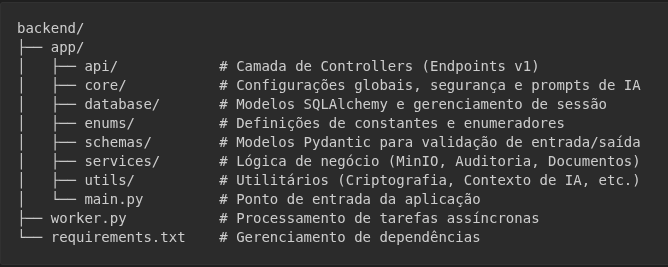
\includegraphics[width=0.5\linewidth]{images/Estrutura-backend.png}
    \caption{Diagrama de Arquitetura do Sistema. Fonte: Autor}
    \label{fig:Representação da estrutura de diretórios do backend da plataforma.}
\end{figure}

\begin{itemize}

\item \textbf{app/api}: contém a definição das rotas da API e os controladores responsáveis por receber as requisições do frontend.

\item \textbf{app/core}: armazena configurações globais da aplicação, incluindo parâmetros de segurança, autenticação e inicialização do sistema.

\item \textbf{app/database}: contém os modelos de dados definidos com SQLAlchemy, bem como a configuração de conexão com o banco de dados.

\item \textbf{app/schemas}: define os modelos de dados utilizados para validação de entrada e saída das requisições da API, utilizando a biblioteca Pydantic.

\item \textbf{app/services}: implementa a lógica de negócio do sistema, incluindo geração de documentos, integração com APIs externas e manipulação de dados clínicos.

\item \textbf{app/utils}: reúne funções auxiliares relacionadas à manipulação de arquivos, criptografia, integração com inteligência artificial e comunicação com serviços externos.

\end{itemize}

\subsection{MinIO}

Para a persistência de arquivos binários, como documentos em \textit{PDF} gerados pela plataforma e anexos enviados pelos usuários, foi integrada a solução de armazenamento de objetos \textit{MinIO}. O \textit{MinIO} é um servidor de armazenamento de alto desempenho, compatível com a \textit{API Amazon S3}, que permite o armazenamento de dados não estruturados de forma escalável e segura.

No contexto do sistema \textit{NaraPsi}, o \textit{MinIO} opera em um \textit{container Docker} dedicado, sendo acessado pelo \textit{backend} através da biblioteca \textit{boto3} (cliente \textit{SDK} para serviços compatíveis com \textit{S3}). A arquitetura de armazenamento foi organizada em \textit{buckets} distintos: um destinado aos documentos clínicos gerados (\textit{MINIO\_BUCKET\_NAME\_DOCS}) e outro para anexos diversos (\textit{MINIO\_BUCKET\_NAME\_ANEXOS}).

Visando a segurança dos dados em repouso (\textit{Data-at-Rest}), o \textit{MinIO} foi configurado com suporte a \textit{SSE} (\textit{Server-Side Encryption}), garantindo que os objetos sejam criptografados automaticamente antes de serem escritos no disco físico. A integração na camada de serviço (\textit{app/services/minio.py}) abstrai as operações de \textit{upload}, \textit{download} e exclusão, vinculando o identificador do objeto (\textit{Key}) ao registro correspondente na base de dados relacional \textit{MySQL}.

\section{Modelagem do Banco de Dados}

A modelagem do banco de dados foi elaborada com base nos requisitos funcionais, regras de negócio e fluxos de informação definidos nas etapas anteriores do projeto. O objetivo principal é garantir a integridade, a segurança e a rastreabilidade dos dados sensíveis relacionados aos pacientes e documentos terapêuticos. O modelo foi estruturado para suportar a associação entre psicólogos e seus respectivos pacientes, o controle de documentos em diferentes estados (em elaboração e finalizado), bem como o registro de assinaturas digitais obrigatórias.

O sistema utiliza o banco de dados relacional MySQL, escolhido por sua robustez, ampla documentação, suporte à integridade referencial e compatibilidade com práticas modernas de desenvolvimento web. A modelagem contempla ainda aspectos de segurança como criptografia de dados sensíveis e registros de log para ações críticas, atendendo às exigências da Lei Geral de Proteção de Dados (LGPD). A seguir, apresenta-se o diagrama relacional que representa as principais entidades e seus relacionamentos.

\subsection{Schema Principal}

O schema principal é responsável por centralizar toda a operação clínica e administrativa do sistema. Ele é estruturado em torno do gerenciamento de identidades, com tabelas base como \texttt{pessoas}, \texttt{usuarios}, \texttt{psicologos} e a tabela associativa \texttt{pacientes\_psicologos}, que define o vínculo terapêutico. 

O controle de acesso é gerenciado de forma granular por meio das tabelas de \texttt{perfis}, \texttt{modulos} e \texttt{regras}, permitindo um sistema de permissões baseado em papéis (RBAC). No âmbito do prontuário eletrônico, o schema armazena registros detalhados nas tabelas de \texttt{sessoes}, \texttt{anamneses}, \texttt{documentos} e \texttt{anexos}, além de gerenciar a comunicação na tabela \texttt{historicos\_chats}. Destaca-se também o robusto sistema de documentação, que inclui a geração de textos a partir de \texttt{templates} com variáveis dinâmicas (\texttt{variaveis\_template}) e o controle do ciclo de vida das \texttt{assinaturas} eletrônicas via integrações de envelopes. A integridade dos dados é mantida por meio de restrições rígidas de chaves estrangeiras com exclusão em cascata (\textit{ON DELETE CASCADE}) para dados dependentes.

\begin{figure}[H]
    \centering
    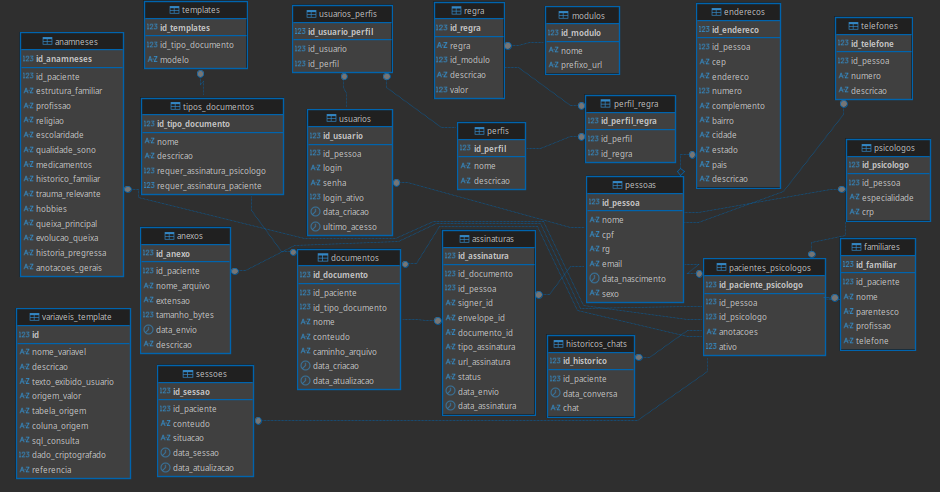
\includegraphics[width=\textwidth]{images/modelo_relacional_banco_schema_principal.png}
    \caption{Diagrama Entidade-Relacionamento do Schema Principal. Fonte: Autor}
    \label{fig:schema_principal}
\end{figure}

\subsection{Schema de Auditoria}

O schema de auditoria foi desenhado como um banco de dados independente (\texttt{auditoria}) para atuar como uma camada de segurança paralela, garantindo o fiel cumprimento das normas de privacidade e da LGPD. Ele é composto fundamentalmente pela tabela \texttt{eventos\_auditoria}, que registra detalhadamente qualquer interação com o sistema.

Cada registro de log armazena metadados essenciais, como o \textit{timestamp} da ação, identificação do usuário, perfil de acesso, IP de origem e a ação específica realizada (\textit{CREATE, UPDATE, DELETE, VIEW}, entre outras). Para assegurar a rastreabilidade completa das modificações, o sistema salva os valores anteriores e os novos valores da entidade afetada. Visando garantir a imutabilidade e a proteção contra fraudes internas, a modelagem implementa uma cadeia de hashes criptográficos (\texttt{hash\_evento} e \texttt{hash\_anterior}). Além disso, foram criados \textit{Triggers} (Gatilhos) diretamente no nível do banco de dados que bloqueiam explicitamente qualquer tentativa de \texttt{UPDATE} ou \texttt{DELETE} na tabela de logs, tornando os registros permanentes e invioláveis.

\begin{figure}[H]
    \centering
    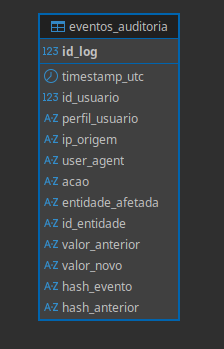
\includegraphics[width=0.3\textwidth]{images/modelo_relacional_banco_schema_auditoria.png} % Ajuste o valor 0.8 conforme necessário
    \caption{Diagrama Entidade-Relacionamento do Schema de Auditoria. Fonte: Autor}
    \label{fig:schema_auditoria}
\end{figure}

\section{Integração de Inteligência Artificial}

A integração de inteligência artificial no sistema NaraPsi visa auxiliar o profissional na elaboração de documentos e na extração de informações de prontuários.

\subsection{Geração Automatizada}

Quando o modelo de documento possui campos configurados para geração automática por inteligência artificial, o sistema injeta o contexto clínico do paciente — recuperado a partir da anamnese e do histórico consolidado de sessões — no \textit{template} de entrada (\textit{prompt}) do modelo. A consulta ao \textit{LLM} é gerenciada pela classe \textit{agenteIA}, que utiliza parâmetros de geração como \textit{n\_ctx} para dimensionamento da janela de contexto e \textit{n\_threads} para paralelismo computacional.

Esta funcionalidade permite que trechos textuais complexos, como sínteses de sessões ou sugestões de encaminhamento, sejam pré-redigidos pela IA com base nas informações já registradas, reduzindo a carga administrativa do psicólogo.

\section{Funcionamento das Principais Funcionalidades}

O sistema NaraPsi possui diversas funcionalidades voltadas para apoiar o trabalho clínico dos psicólogos e otimizar a gestão de informações dos pacientes. Entre as funcionalidades mais relevantes destacam-se a geração automatizada de documentos terapêuticos e o sistema de auditoria de dados.

A geração automatizada de documentos clínicos ocorre a partir de modelos previamente cadastrados no sistema. Inicialmente, o psicólogo seleciona um modelo de documento, como laudo, relatório ou encaminhamento. Em seguida, o sistema recupera automaticamente as informações necessárias do banco de dados, incluindo dados do paciente, informações do psicólogo e registros clínicos relevantes. Após a geração do conteúdo, o documento é estruturado em formato HTML e posteriormente convertido para PDF utilizando a biblioteca WeasyPrint. O arquivo final é armazenado no serviço de armazenamento de objetos MinIO.

\subsection{Geração e Manipulação de Documentos}

A geração de documentos clínicos é uma das funcionalidades centrais da plataforma NaraPsi. O sistema permite que o psicólogo selecione um modelo de documento previamente cadastrado e realize o preenchimento automático das informações do paciente, podendo ainda utilizar recursos de inteligência artificial para gerar trechos textuais com base no histórico clínico.

A Figura~\ref{fig:fluxo-geracao-documentos} apresenta o fluxo completo de geração, processamento e disponibilização dos documentos terapêuticos no sistema.

\begin{figure}[H]
\centering
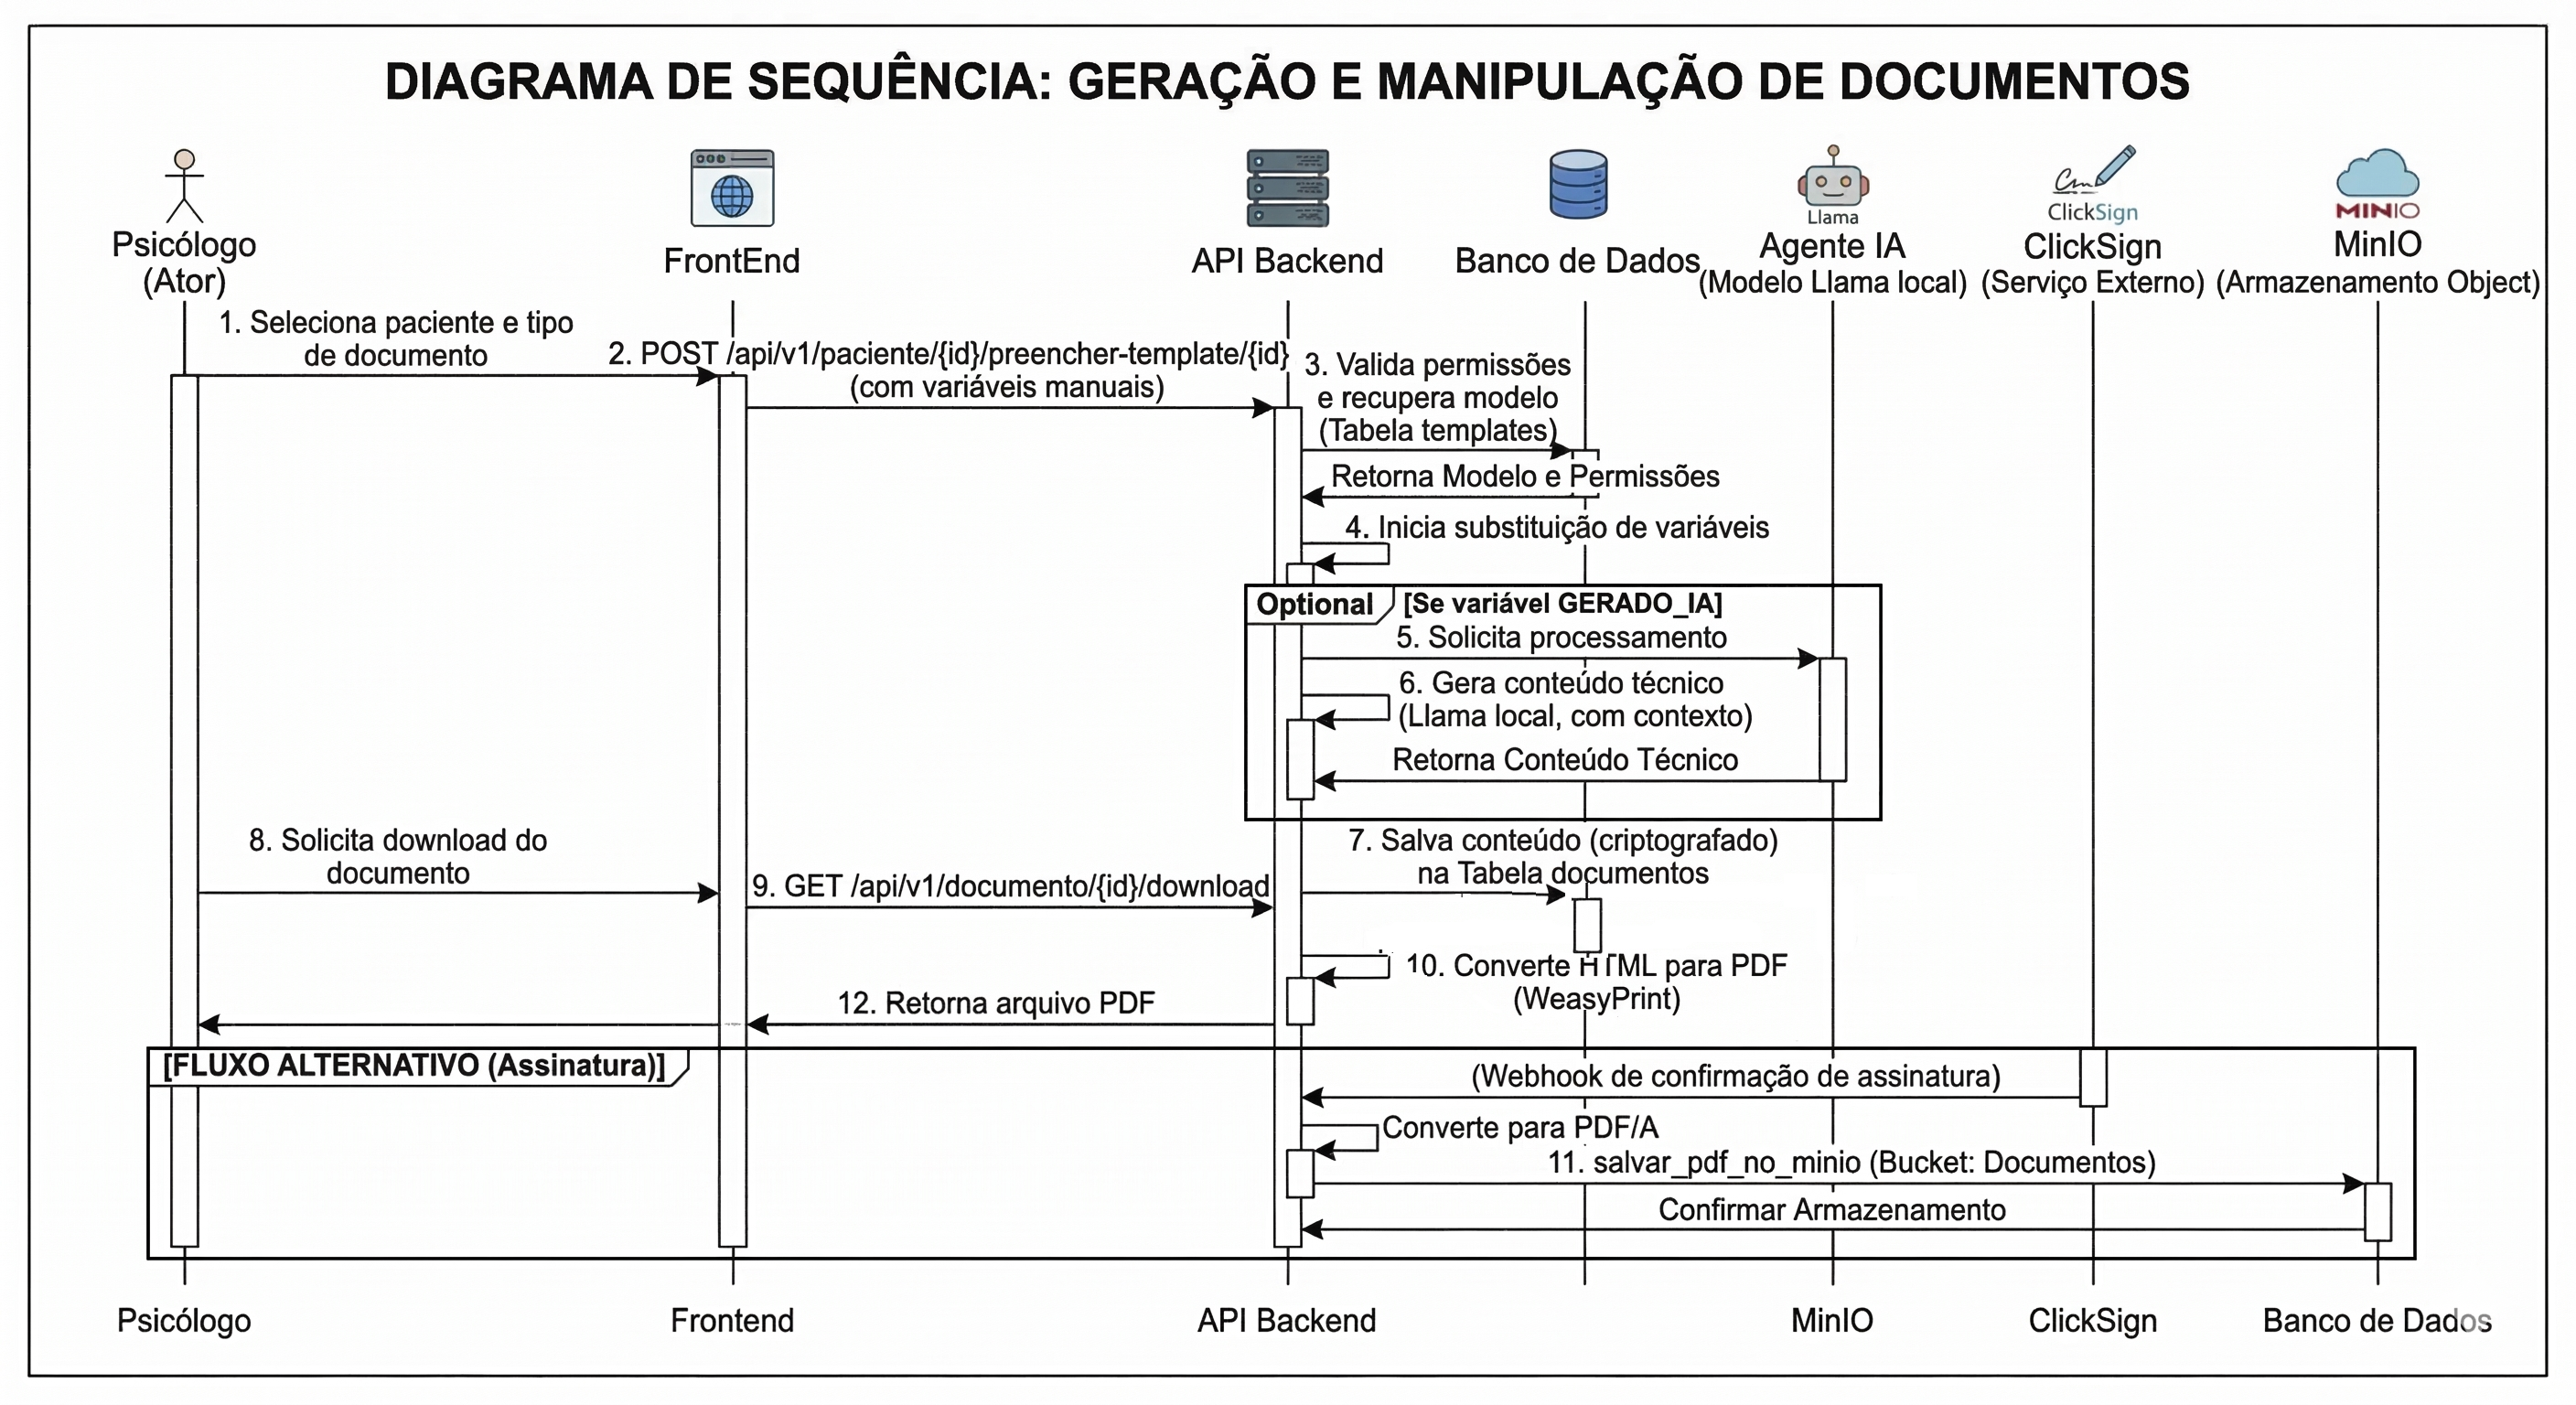
\includegraphics[width=0.9\linewidth]{images/geracao_manipulacao_documentos.png}
\caption{Fluxo de geração e manipulação de documentos clínicos na plataforma NaraPsi. Fonte: Autor}
\label{fig:fluxo-geracao-documentos}
\end{figure}

Conforme ilustrado no diagrama, o processo inicia-se quando o psicólogo seleciona um paciente e o tipo de documento desejado na interface da aplicação. O frontend envia uma requisição ao backend, que valida as permissões do usuário e recupera o modelo de documento armazenado no banco de dados. Durante o preenchimento do template, o sistema substitui variáveis dinâmicas por informações do paciente e, quando configurado, solicita ao agente de inteligência artificial a geração automática de determinados trechos textuais. O conteúdo final é armazenado na base de dados e pode posteriormente ser convertido para o formato PDF por meio da biblioteca WeasyPrint. Em casos onde o documento necessita de assinatura digital, o sistema integra-se à API da plataforma ClickSign e armazena o arquivo final no serviço de armazenamento MinIO.

\subsection{Auditoria}

Considerando a sensibilidade das informações armazenadas, o sistema implementa um mecanismo de auditoria para registrar todas as operações relevantes realizadas na plataforma. Sempre que ocorre uma ação crítica — como criação, alteração ou exclusão de dados — o sistema registra um log contendo informações sobre o usuário responsável, data e hora da operação e os dados envolvidos na modificação.

A Figura~\ref{fig:fluxo-auditoria} apresenta o fluxo de registro e processamento dos logs de auditoria implementado na plataforma.

\begin{figure}[H]
\centering
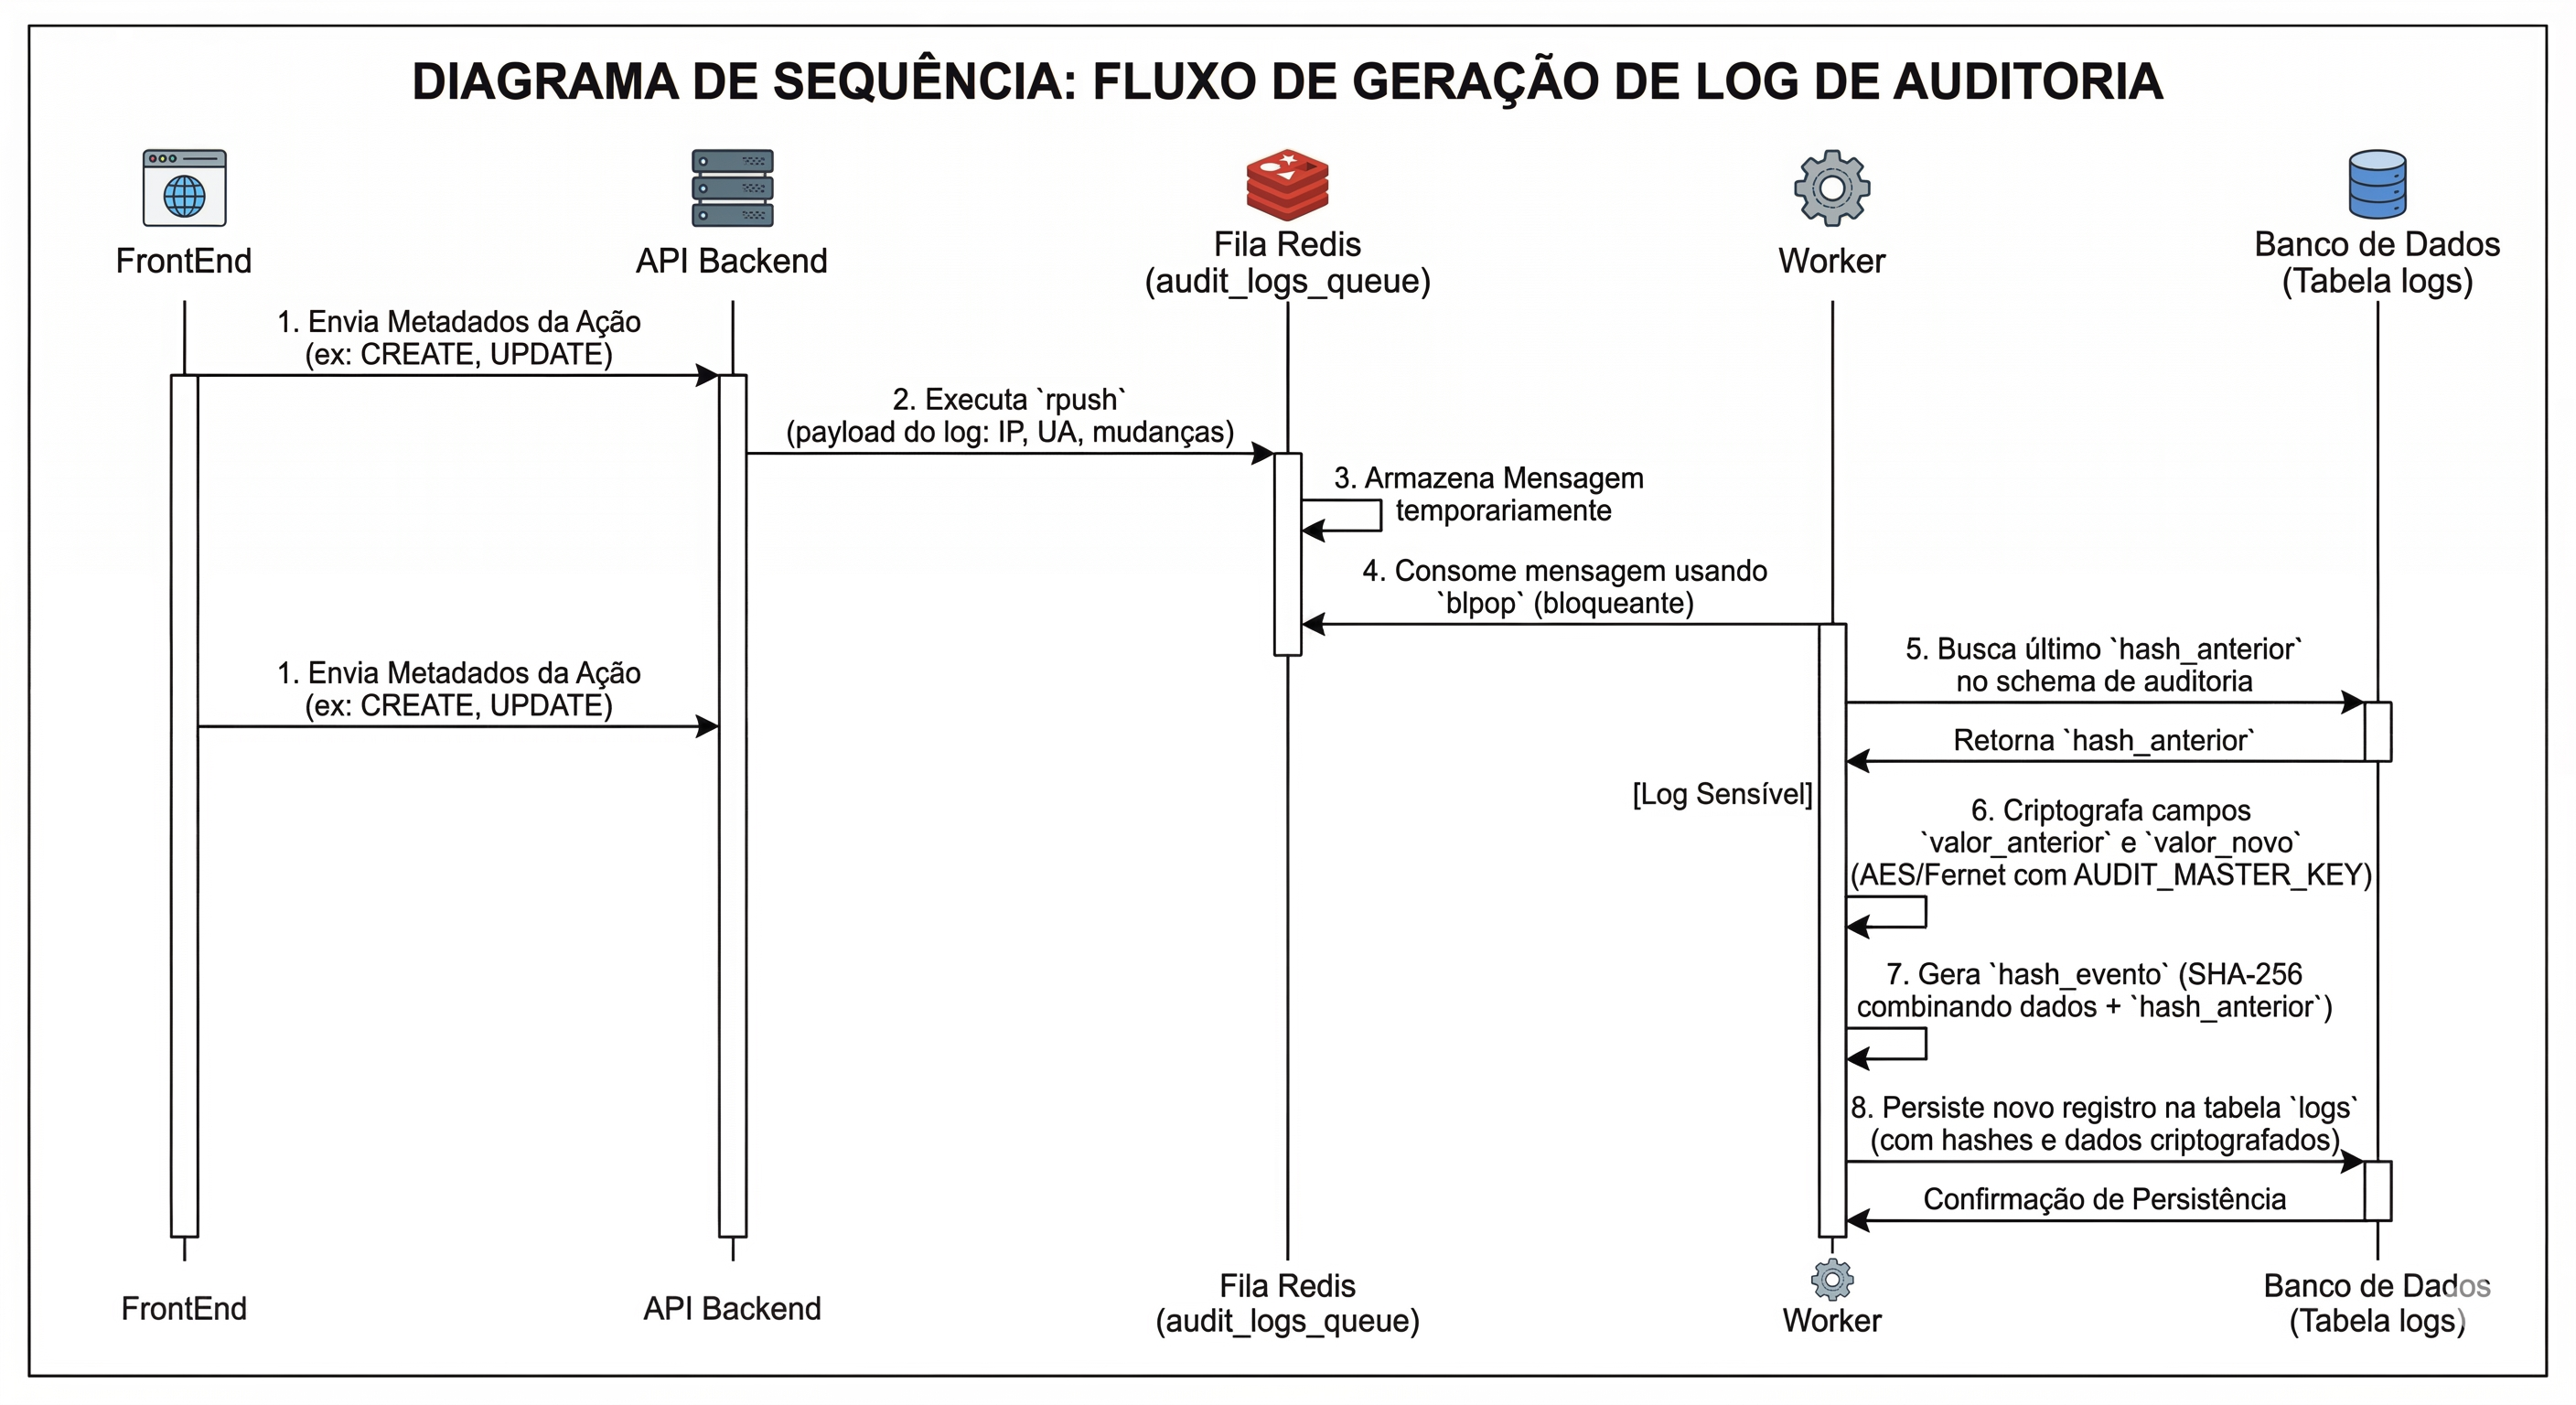
\includegraphics[width=0.9\linewidth]{images/logs auditoria.png}
\caption{Fluxo de gravação e processamento dos logs de auditoria do sistema. Fonte: Autor}
\label{fig:fluxo-auditoria}
\end{figure}

Nesse fluxo, qualquer ação relevante realizada na aplicação — como autenticação, criação, atualização ou exclusão de registros — é interceptada pelo serviço de auditoria do backend. Os metadados do evento são enviados para uma fila Redis, onde ficam temporariamente armazenados até serem processados por um \textit{worker} em segundo plano. O processo de processamento do log inclui a recuperação do último hash registrado, a criptografia de campos sensíveis quando necessário e a geração de um novo hash criptográfico utilizando o algoritmo SHA-256. Por fim, o registro é persistido no banco de dados de auditoria, garantindo a rastreabilidade e a integridade das operações realizadas no sistema.

Os registros de auditoria são criptografados e encadeados utilizando algoritmos de hash SHA-256. Esse mecanismo garante a integridade dos logs, impedindo alterações não autorizadas e permitindo a verificação posterior da autenticidade das informações. Esta abordagem garante maior transparência e segurança no tratamento de dados pessoais sensíveis, estando em conformidade com os princípios estabelecidos pela Lei Geral de Proteção de Dados (LGPD).

\section{Segurança da Informação e LGPD}

Considerando a natureza sensível das informações manipuladas pelo sistema, foram implementados diversos mecanismos de segurança voltados para a proteção dos dados e conformidade com a Lei Geral de Proteção de Dados (LGPD).

Para melhor compreensão do processo de autenticação implementado na plataforma, a Figura~\ref{fig:fluxo-autenticacao} apresenta o diagrama de sequência que descreve o fluxo completo de validação das credenciais, geração do token de acesso e registro do evento de autenticação no sistema.

\begin{figure}[H]
\centering
\includegraphics[width=0.9\linewidth]{images/fluxo_autenticacao.png}
\caption{Fluxo de autenticação da plataforma NaraPsi. Fonte: Autor}
\label{fig:fluxo-autenticacao}
\end{figure}

Conforme ilustrado no diagrama, o processo inicia-se quando o psicólogo insere suas credenciais na interface de login da aplicação. O frontend envia uma requisição ao endpoint de autenticação da API backend, que realiza a validação das credenciais consultando a tabela de usuários no banco de dados. A senha informada é comparada com o hash armazenado utilizando o algoritmo bcrypt. Em caso de validação bem-sucedida, o sistema gera um token JWT contendo o identificador do usuário e atualiza o registro de último acesso. Adicionalmente, um evento de auditoria é enviado para a fila de logs, garantindo o registro da tentativa de autenticação no sistema.

\subsection{Autenticação} 

A autenticação dos usuários é realizada via \textit{Bearer Tokens} no padrão \textit{JWT} (\textit{JSON Web Tokens}). Após a validação das credenciais (\textit{POST /auth/login}), o sistema gera um \textit{token stateless} que encapsula o \textit{payload} de identificação do usuário, permitindo o tráfego seguro de autorizações entre o cliente e o servidor. 

O controle de acesso é implementado sob o paradigma de \textit{RBAC} (\textit{Role-Based Access Control}), onde as permissões são validadas de forma granular através de \textit{middlewares} que verificam os perfis vinculados ao usuário na base de dados relacional.

\subsection{Proteção de Credenciais} 

As senhas dos usuários não são armazenadas em formato de texto plano. O sistema utiliza a técnica de \textit{salting} e \textit{hashing} criptográfico por meio do algoritmo \textit{bcrypt} (via biblioteca \textit{Passlib}), garantindo a resistência contra ataques de dicionário e \textit{rainbow tables}.

\subsection{Integridade de Logs} 

Para garantir a integridade dos registros de auditoria, foi implementado um mecanismo de encadeamento criptográfico (\textit{hash chaining}) processado de forma assíncrona por um \textit{worker} especializado em segundo plano. Cada registro de auditoria possui um \textit{hash} SHA-256 calculado a partir de uma semente que contém os metadados do evento (ID do usuário, ação realizada, entidade afetada) e o \textit{hash} do registro imediatamente anterior.

Caso o evento envolva dados sensíveis (alteração de prontuário, por exemplo), os valores são submetidos a um processo de criptografia simétrica (\textit{Fernet/AES}) antes de serem persistidos na base de dados de auditoria. Matematicamente, o encadeamento é definido pela função recursiva:

\[ H_n = SHA256(S_n + H_{n-1}) \] 

Onde $S_n$ representa a semente serializada do evento $n$ e $H_{n-1}$ o \textit{hash} do evento anterior. Esse modelo garante a imutabilidade lógica dos registros históricos, visto que qualquer alteração em um bloco anterior invalidaria toda a cadeia subsequente.

\section{Interfaces do Sistema}

Esta seção apresenta algumas das principais interfaces do sistema NaraPsi, com o objetivo de demonstrar visualmente as funcionalidades disponibilizadas aos usuários. As telas apresentadas ilustram o fluxo de utilização da plataforma tanto para psicólogos quanto para administradores.

\subsection{Tela de Login}

A Figura~\ref{fig:tela-login} ilustra a interface de autenticação da plataforma NaraPsi. O processo de controle de acesso foi implementado utilizando o protocolo HTTP aliado ao padrão de tokens \textit{stateless}. Ao submeter suas credenciais, o sistema realiza uma requisição cifrada ao \textit{backend}, que valida a identidade do usuário contra os \textit{hashes} armazenados no banco de dados.

Após a validação bem-sucedida, o servidor retorna um \textit{JSON Web Token} (JWT). Para garantir a persistência da sessão e permitir a navegação entre as diferentes rotas da aplicação sem a necessidade de novos \textit{logins}, este token, juntamente com dados não sensíveis de perfil (como nome e nível de acesso), é armazenado no \textbf{LocalStorage} do navegador do cliente.

Esta abordagem permite que o \textit{frontend} anexe o token automaticamente ao cabeçalho de autorização (\textit{Authorization Header}) de todas as requisições subsequentes via protocolo TLS, assegurando a integridade e a autenticidade da comunicação. Além disso, a gestão via \textit{LocalStorage} possibilita que o estado da aplicação seja mantido mesmo após o fechamento ou atualização da aba do navegador, otimizando a experiência de uso do profissional.

\begin{figure}[H]
    \centering
    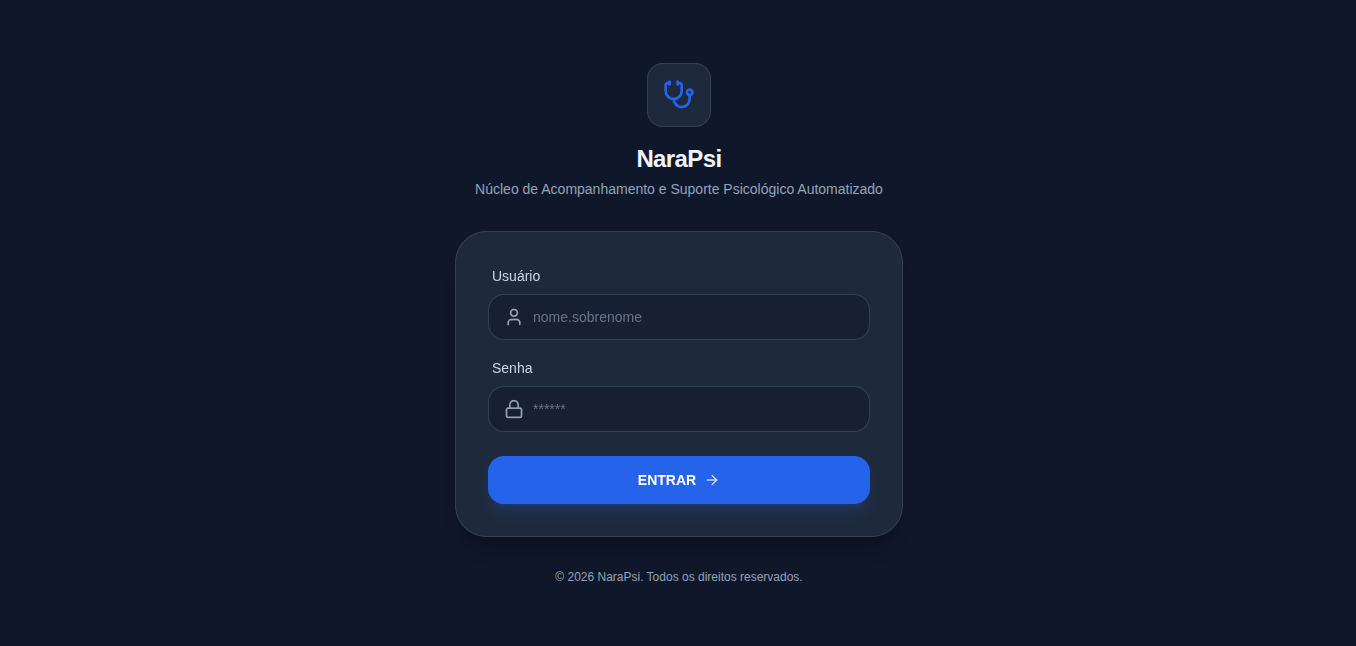
\includegraphics[width=0.8\linewidth]{images/tela_login.png}
    \caption{Tela de autenticação do sistema NaraPsi. Fonte: Autor}
    \label{fig:tela-login}
\end{figure}


\subsection{Dashboard do Psicólogo}

A Figura~\ref{fig:dashboard-psicologo} ilustra a interface principal da plataforma, denominada \textit{Dashboard}, visualizada pelo profissional logo após a autenticação. O painel foi projetado para oferecer uma visão consolidada e imediata de dados relevantes à gestão clínica, utilizando elementos gráficos que facilitam a interpretação rápida das informações.

No centro da interface, destaca-se um componente de visualização de dados do tipo gráfico de rosca (donut chart), que apresenta a distribuição demográfica dos pacientes atendidos, segmentada por gênero. À direita, o sistema exibe um módulo de notificações e lembretes, como o quadro de "Aniversariantes do Dia", que auxilia o profissional na manutenção do vínculo terapêutico e na gestão da agenda.

\begin{figure}[H]
    \centering
    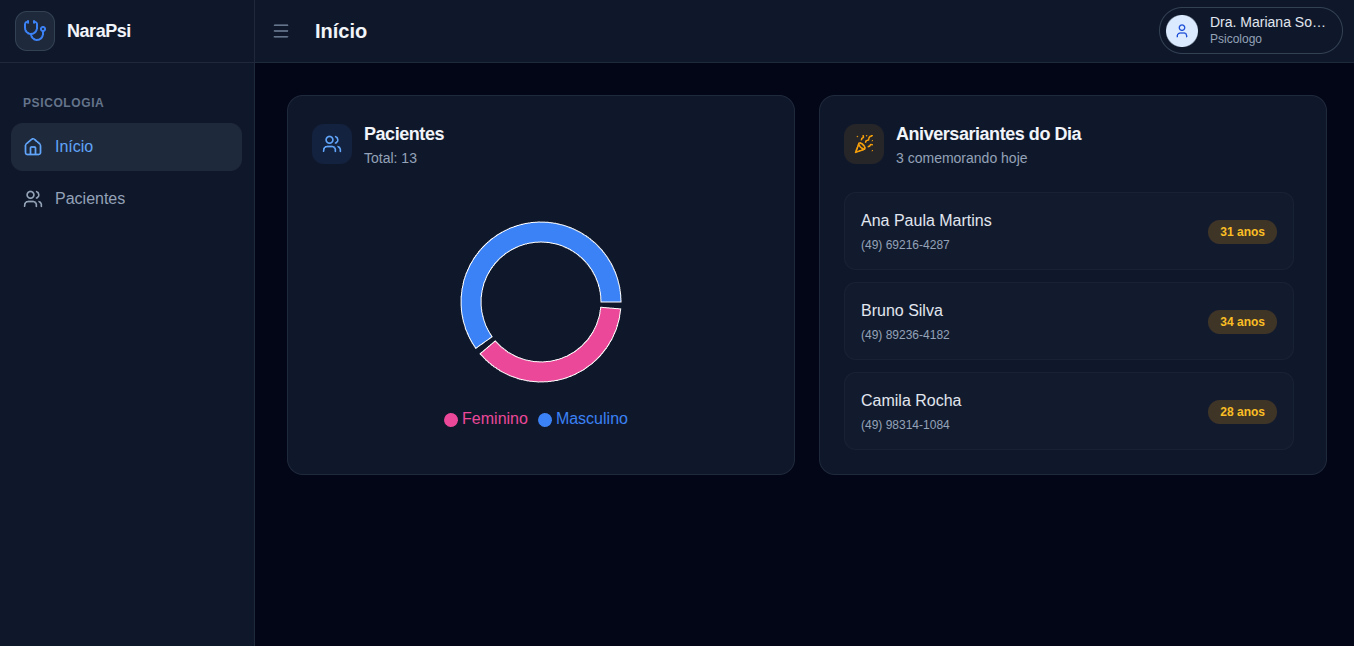
\includegraphics[width=0.9\linewidth]{images/dash_psicologo.png}
    \caption{Dashboard do psicólogo na plataforma NaraPsi. Fonte: Autor}
    \label{fig:dashboard-psicologo}
\end{figure}


\subsection{Gestão de Pacientes}

A Figura~\ref{fig:pacientes-psicologo} ilustra a interface de gerenciamento de pacientes, componente central para o fluxo de trabalho clínico na plataforma NaraPsi. Esta tela foi projetada utilizando o padrão de tabelas de dados (data tables), permitindo uma visualização estruturada e cronológica dos indivíduos sob acompanhamento.

A fim de aprimorar a usabilidade da interface, foi implementado um campo de busca dinâmica na parte superior da tela, possibilitando a filtragem de registros em tempo real com base no nome informado pelo usuário.

Cada linha da tabela apresenta atributos essenciais: identificação do paciente, sexo (com auxílio de etiquetas visuais coloridas para rápida distinção), idade e a data da última sessão realizada. Caso não existam atendimentos registrados, o sistema sinaliza o estado como "Sem sessões". À direita, a coluna de ações fornece o ponto de entrada para o prontuário eletrônico completo, onde o profissional pode acessar o histórico detalhado, realizar o \textit{upload} de documentos via MinIO ou iniciar a geração de novos registros terapêuticos assistidos por Inteligência Artificial.

\begin{figure}[H]
    \centering
    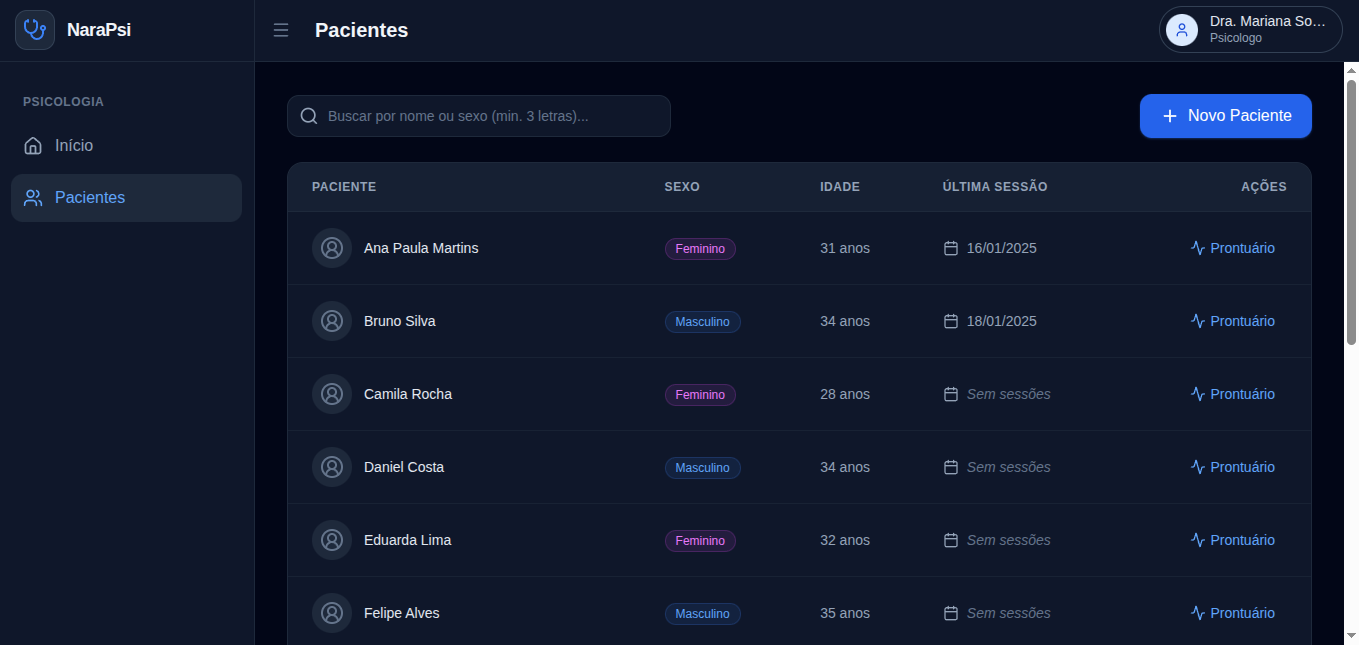
\includegraphics[width=0.9\linewidth]{images/pacientes_psicologo.png}
    \caption{Tela de gerenciamento de pacientes. Fonte: Autor}
    \label{fig:pacientes-psicologo}
\end{figure}


\subsection{Prontuário do Paciente}

A Figura~\ref{fig:prontuario} detalha a interface do prontuário eletrônico, concebida sob uma arquitetura de componentes modulares para centralizar o histórico clínico do paciente. No cabeçalho da página, o sistema apresenta um \textit{card} de identificação com dados biográficos e de contato, além de atalhos para a edição cadastral e para a realização da anamnese, garantindo que as informações primordiais estejam sempre acessíveis.

A organização das informações clínicas é dividida em três contêineres principais:

\begin{itemize}
\item \textbf{Sessões Terapêuticas:} Implementa uma lista cronológica reversa dos atendimentos. É possível observar o gerenciamento de estados do documento (RN03); a "Sessão \#8" apresenta o status "EDITANDO", permitindo alterações, enquanto a "Sessão \#1" figura como "CONCLUÍDO", indicando a imutabilidade do registro e disponibilizando opções de visualização e \textit{download} em PDF.
\item \textbf{Documentos:} Área destinada à gestão de arquivos gerados pela plataforma (laudos, pareceres e encaminhamentos), integrando as funcionalidades de Inteligência Artificial e assinatura digital.
\item \textbf{Arquivos Anexados:} Módulo responsável pela interface com o serviço de armazenamento de objetos MinIO, permitindo a gestão de documentos externos e exames complementares de forma segura.
\end{itemize}

O \textit{design} utiliza elementos de \textit{feedback} visual, como etiquetas de status coloridas e ícones intuitivos para ações de CRUD (\textit{Create, Read, Update, Delete}), assegurando que o psicólogo tenha controle total sobre o fluxo documental de forma ergonômica e em conformidade com os requisitos de segurança e integridade de dados estabelecidos.

\begin{figure}[H]
    \centering
    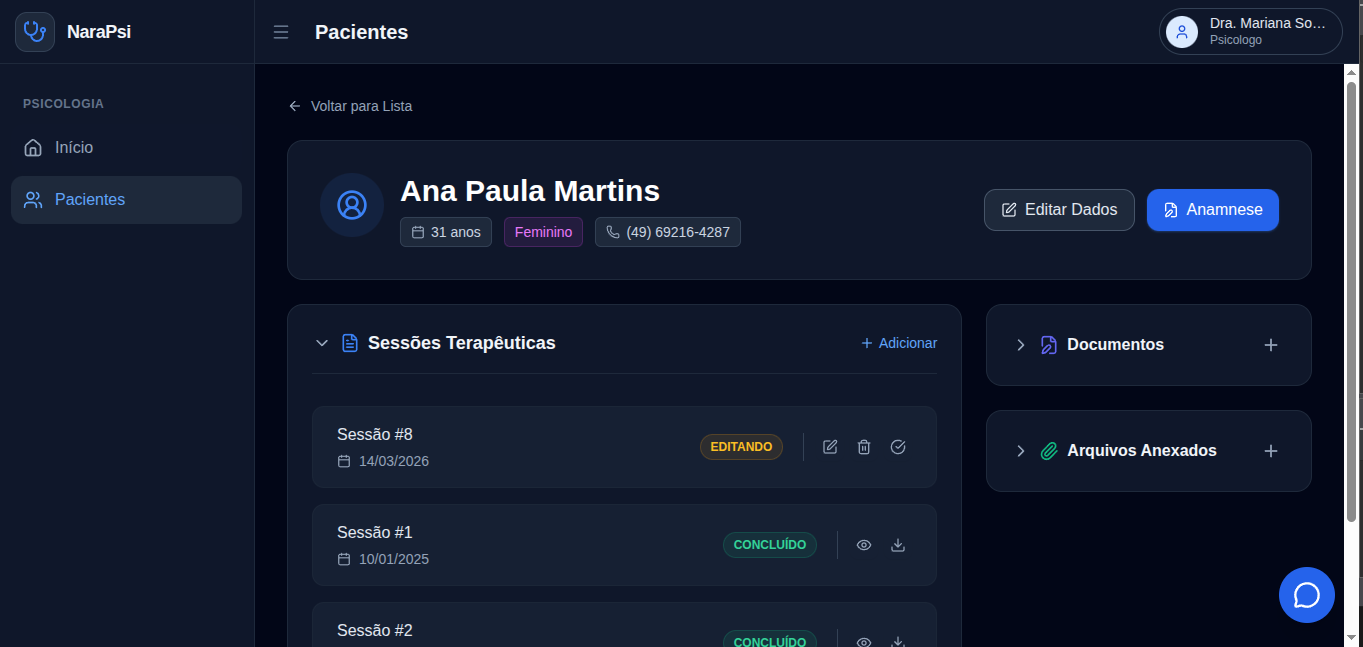
\includegraphics[width=0.9\linewidth]{images/prontuário_psicologo.png}
    \caption{Interface de prontuário clínico do paciente. Fonte: Autor}
    \label{fig:prontuario}
\end{figure}


\subsection{Assistente de Inteligência Artificial (Nara IA)}

A Figura~\ref{fig:assistente-ia} ilustra a interface do assistente virtual inteligente, denominado Nara IA, integrado de forma contextual ao prontuário do paciente. Diferente de ferramentas de chat genéricas, este componente foi projetado como um agente especializado que opera exclusivamente sobre o conjunto de dados clínicos do paciente em visualização, respeitando o isolamento de dados entre diferentes prontuários.

A interface utiliza o padrão de \textit{chatbot} para permitir que o psicólogo realize consultas em linguagem natural sobre o histórico terapêutico. No exemplo apresentado, observa-se a capacidade do sistema em realizar o processamento de linguagem natural (NLP) para extrair informações específicas, como a "queixa principal", a partir de múltiplos relatos de sessões anteriores, sem que o profissional precise realizar uma leitura manual exaustiva de todo o histórico.

Tecnicamente, o componente implementa uma arquitetura de \textit{prompting} que concatena os dados clínicos anonimizados ao modelo de linguagem local (Mistral/Llama), garantindo que a resposta seja fundamentada apenas em evidências registradas no sistema. Adicionalmente, a interface exibe um aviso de isenção de responsabilidade (\textit{disclaimer}) destacando que a ferramenta atua como um sistema de apoio à decisão, mantendo a responsabilidade final da validação clínica sob o profissional de saúde, conforme estabelecido na regra de negócio.

\begin{figure}[H]
    \centering
    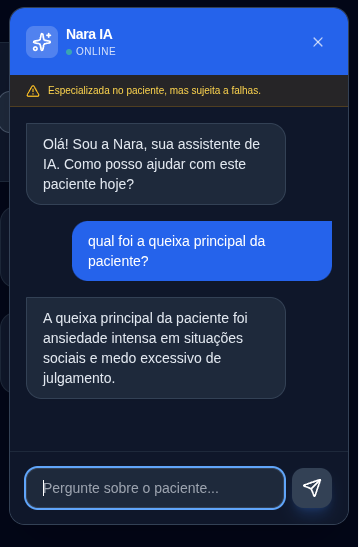
\includegraphics[width=0.3\linewidth]{images/assistente_ia.png}
    \caption{Interface do assistente de inteligência artificial da plataforma. Fonte: Autor}
    \label{fig:assistente-ia}
\end{figure}


\subsection{Dashboard Administrativo e Gestão de Governança}

A Figura~\ref{fig:dashboard-admin} ilustra o painel de controle destinado ao ator Administrador, projetado para fornecer uma visão macroestatística e operacional da plataforma NaraPsi. Esta interface foca na métrica de uso e na integridade da base de usuários, apresentando indicadores consolidados como o total de profissionais de psicologia cadastrados e o volume global de pacientes gerenciados pela aplicação.

A navegação lateral esquerda é segmentada em módulos específicos de governança, permitindo o acesso às funcionalidades de:

\begin{itemize}
\item \textbf{Gestão de Usuários:} Módulo central para o monitoramento de contas. Nesta área, o administrador pode auditar informações críticas como a data de criação da conta, o \textit{status} atual (ativo/inativo), os perfis vinculados e o carimbo de tempo (\textit{timestamp}) do último acesso realizado. A interface oferece ainda controles para a inativação lógica de usuários e a atribuição dinâmica de novos perfis de acesso.
\item \textbf{Gestão de Perfis:} Ambiente destinado à configuração de permissões e papéis dentro do sistema.
\item \textbf{Cadastro de Psicólogos:} Fluxo específico para o ingresso de novos profissionais na plataforma, garantindo a validação de credenciais institucionais antes da liberação do ambiente clínico.
\end{itemize}

Ressalta-se que, em conformidade com o sigilo terapêutico e as regras de negócio estabelecidas, o administrador possui acesso estritamente administrativo. Embora possa gerenciar o ciclo de vida das contas e monitorar logs de atividade para fins de auditoria, o sistema implementa barreiras lógicas que impedem este ator de visualizar o conteúdo sensível dos prontuários ou documentos gerados pelos psicólogos.
\begin{figure}[H]
    \centering
    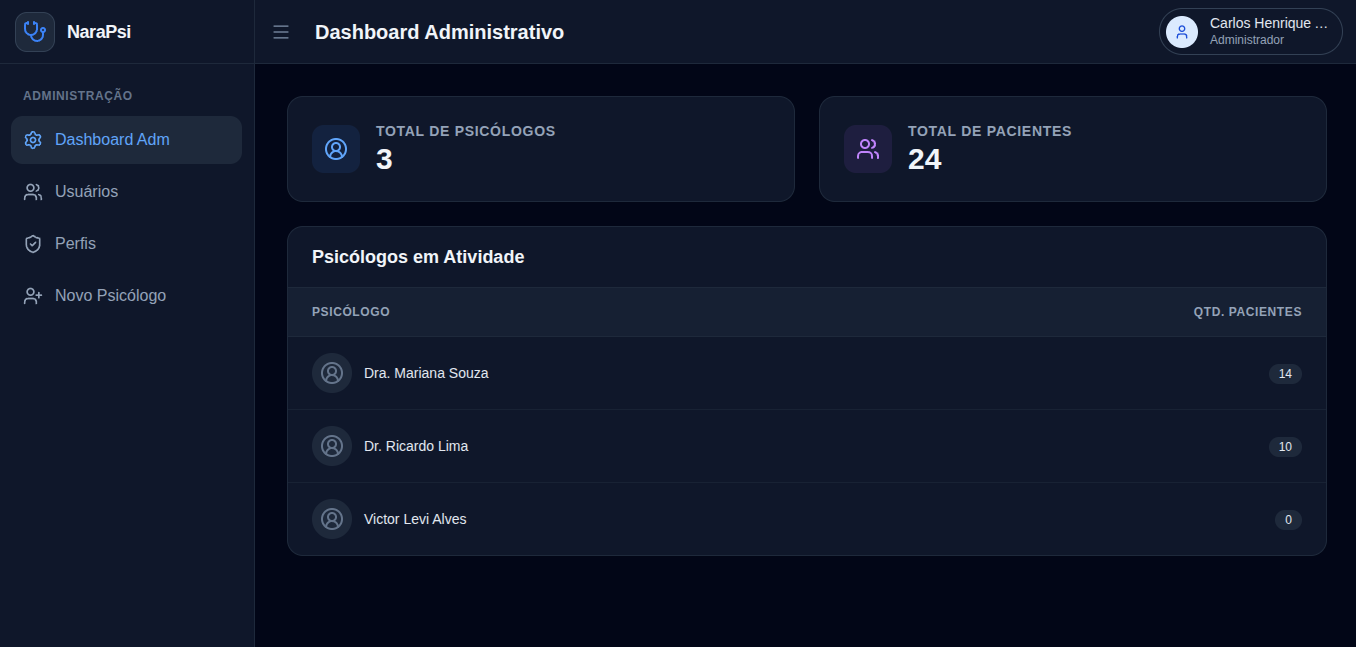
\includegraphics[width=0.9\linewidth]{images/dashboard_administrativo.png}
    \caption{Dashboard administrativo da plataforma. Fonte: Autor}
    \label{fig:dashboard-admin}
\end{figure}


\subsection{Gerenciamento de Identidades e Acessos}

A Figura~\ref{fig:usuarios-admin} detalha a interface de gerenciamento de identidades, onde o administrador operacionaliza o controle de acesso à plataforma. A tela utiliza uma estrutura de listagem dinâmica que oferece uma visão transparente sobre a base de usuários cadastrados, facilitando processos de auditoria e manutenção de contas.

Os principais elementos técnicos e funcionais desta interface incluem:

\begin{itemize}
\item \textbf{Monitoramento de Estado e Atividade:} Para cada registro, o sistema exibe de forma clara o \textit{status} operacional (Ativo/Inativo) por meio de indicadores visuais coloridos, além de registrar a data de criação da conta e o \textit{timestamp} exato do último acesso. Esses dados são fundamentais para a detecção de contas inativas ou comportamentos de acesso anômalos.
\item \textbf{Granularidade de Perfis:} A coluna "Perfis" demonstra a implementação do modelo multi-perfil da plataforma. É possível observar casos em que um mesmo usuário (como exemplificado na "Dra. Mariana Souza") acumula papéis de Administrador, Psicólogo e Paciente, validando a flexibilidade da lógica de permissões baseada em RBAC (\textit{Role-Based Access Control}) descrita anteriormente.
\item \textbf{Ações de Manutenção:} Através do botão "Editar", o administrador acessa o fluxo de modificação de atributos, permitindo a atualização de credenciais institucionais, redefinição de permissões ou a inativação lógica do usuário, garantindo que o ciclo de vida da identidade seja gerido de ponta a ponta.
\end{itemize}

O design da tela prioriza a densidade de informação sem comprometer a legibilidade, utilizando ícones e agrupamentos visuais que permitem ao administrador gerir uma base crescente de usuários com eficiência e precisão técnica.

\begin{figure}[H]
    \centering
    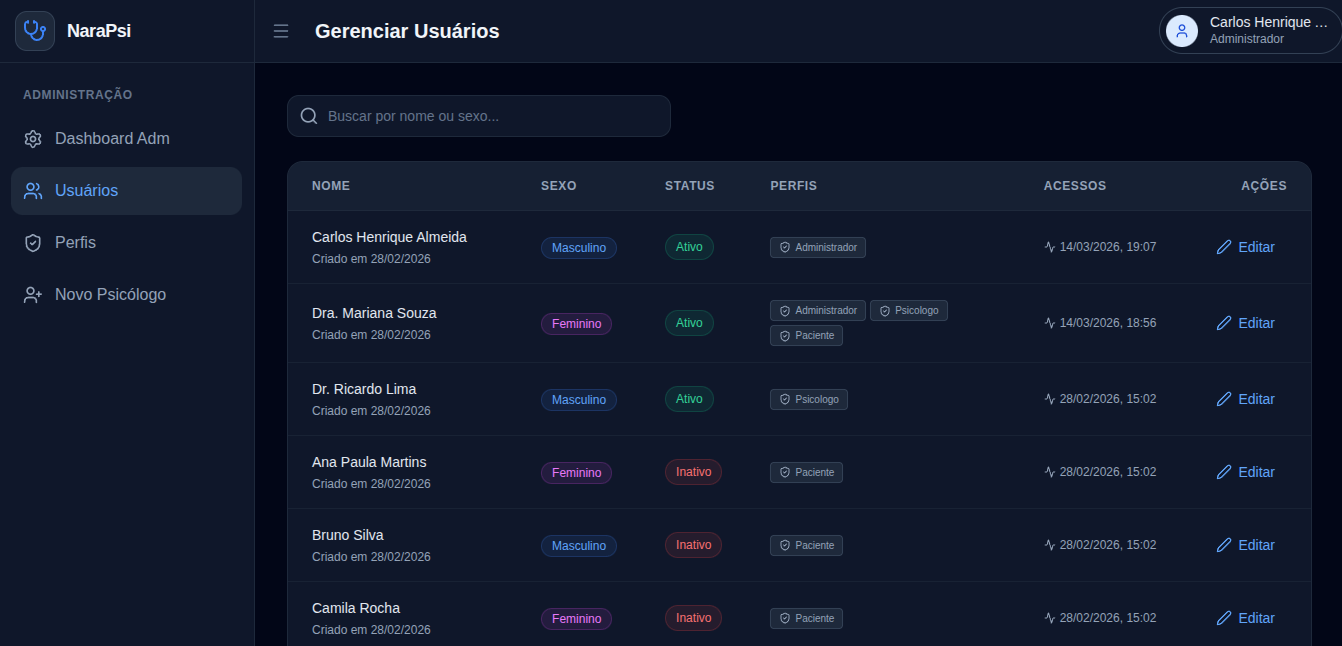
\includegraphics[width=0.9\linewidth]{images/usuários_adm.png}
    \caption{Interface de gerenciamento de usuários da plataforma. Fonte: Autor}
    \label{fig:usuarios-admin}
\end{figure}

\section{Diagramas}

Os diagramas produzidos nesta seção visam ilustrar a arquitetura, o comportamento e a estrutura da plataforma.

\subsection{Arquitetura}

A aplicação é estruturada em três camadas principais: Frontend, Backend e serviços externos. A comunicação entre o cliente (React) e o servidor (FastAPI) ocorre por meio do protocolo seguro HTTPS/TLS. Os dados sensíveis dos pacientes são persistidos no banco \textit{MySQL} utilizando criptografia simétrica \textit{AES} em repouso (nível de aplicação). Os arquivos anexados e os documentos também são criptografados e salvos no \textit{MinIO}. O backend integra com uma API de assinatura digital (ClicSign) e utiliza uma IA local baseada no modelo Mistral para auxiliar na geração de conteúdos clínicos. Todo o fluxo respeita as diretrizes da LGPD.

\begin{figure}[H]
    \centering
    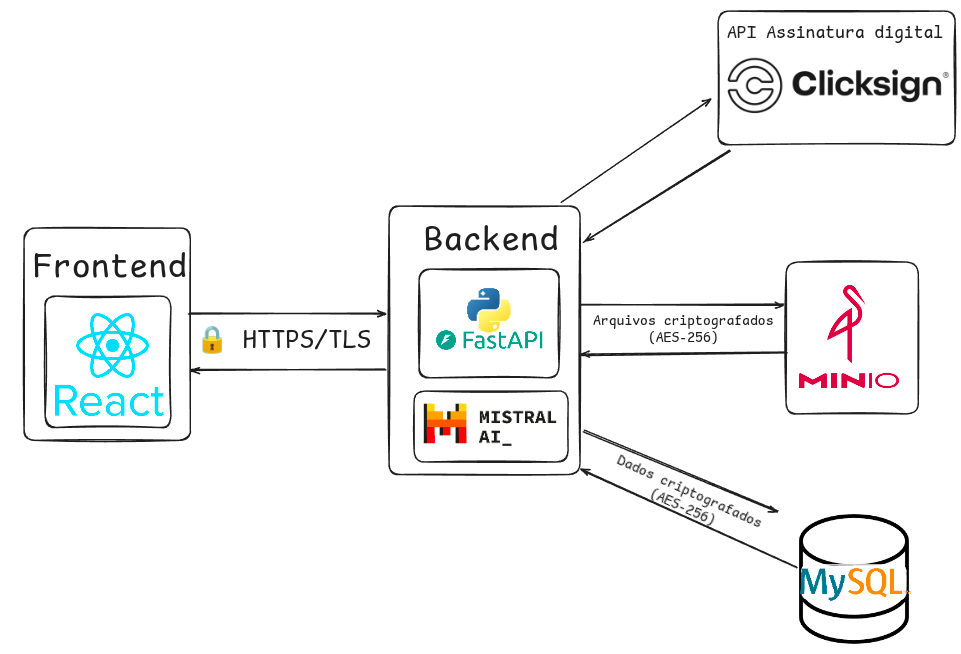
\includegraphics[width=0.5\linewidth]{images/Diagrama de Arquitetura do Sistema.png}
    \caption{Diagrama de Arquitetura do Sistema. Fonte: Autor}
    \label{fig:Diagrama-Arquitetura-Sistemal}
\end{figure}

\subsection{Caso de Uso}

O diagrama de casos de uso tem como objetivo representar as interações entre os atores e o sistema, evidenciando as funcionalidades oferecidas pela plataforma. Na Figura~\ref{fig:Diagrama-caso-uso} apresenta-se o diagrama de casos de uso, onde é possível visualizar as funcionalidades organizadas de acordo com os atores envolvidos.

\begin{figure}[H]
    \centering
    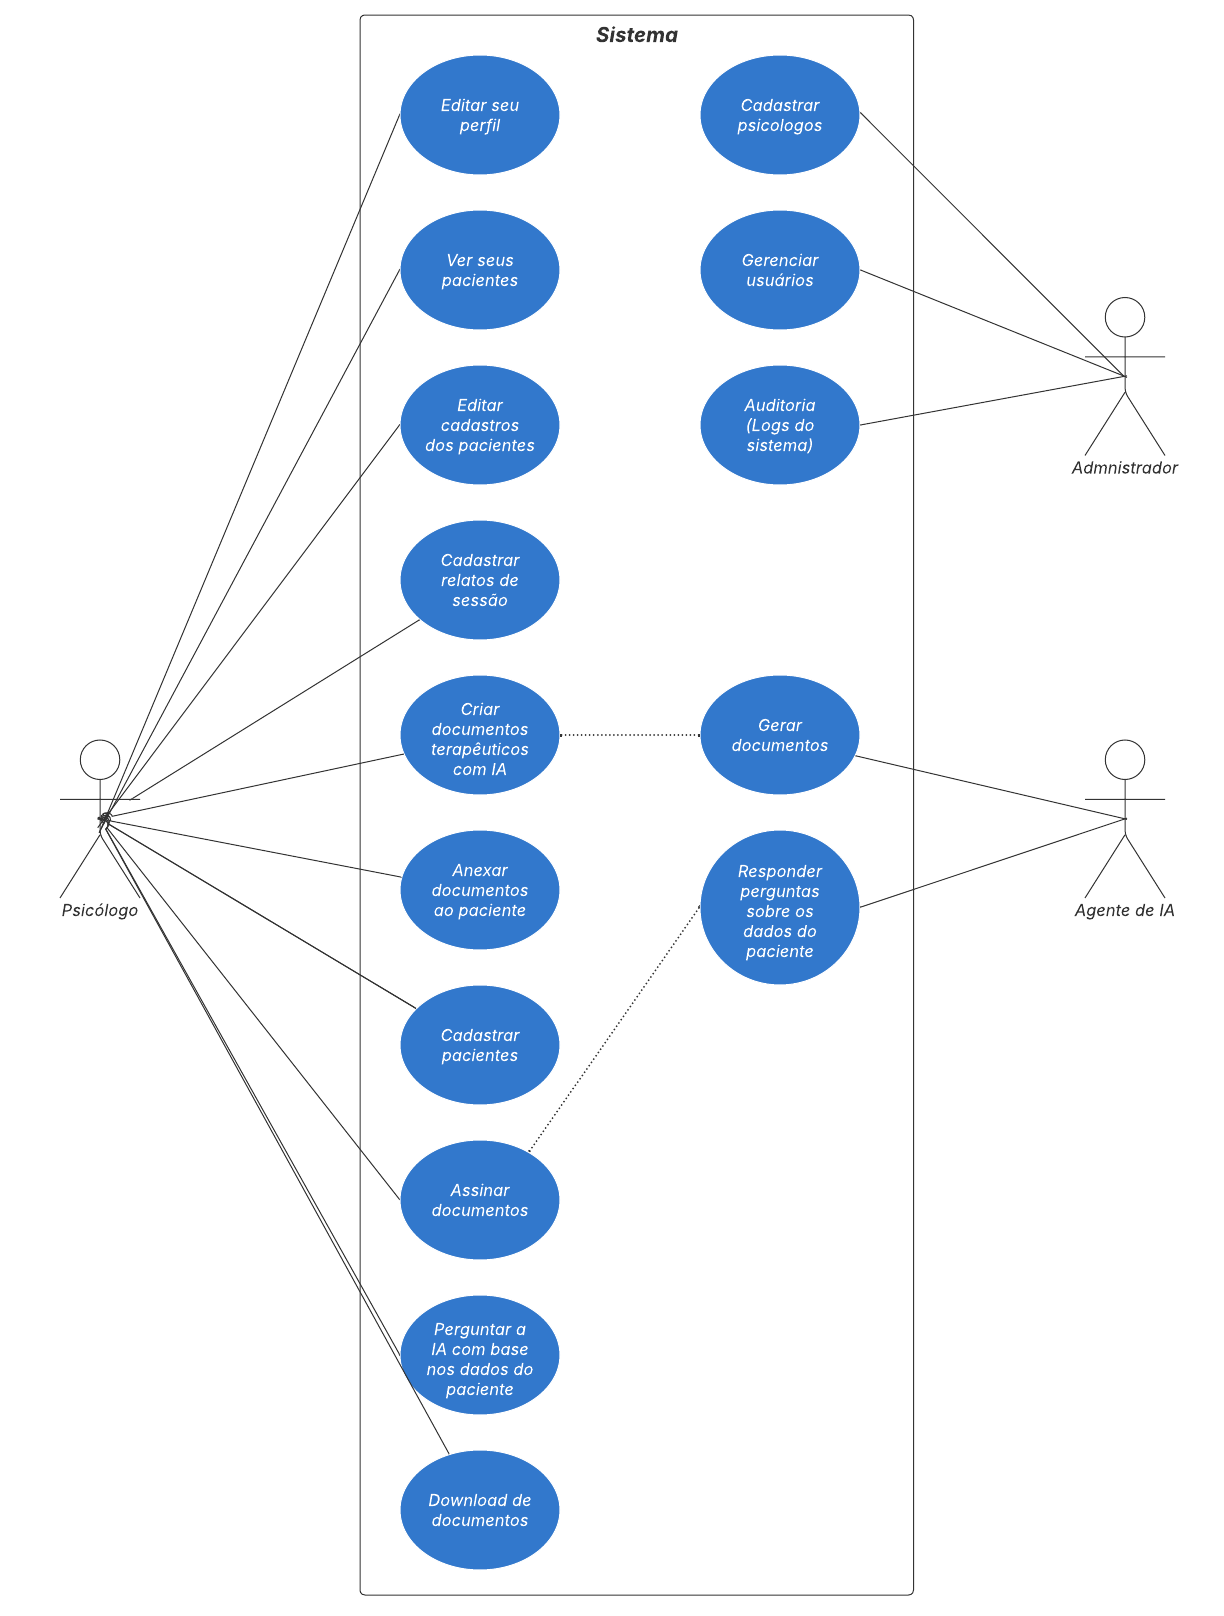
\includegraphics[width=0.5\linewidth]{images/Diagrama de caso de uso.png}
    \caption{Diagrama de Caso de Uso. Fonte: Autor}
    \label{fig:Diagrama-caso-uso}
\end{figure}

\section{Testes e Resultados}

Cada funcionalidade implementada passou por ciclos de testes unitários e testes de integração, com o objetivo de garantir a correta execução das operações e a integridade das informações manipuladas pelo sistema. Ainda por definir melhor os detalhes dos resultados obtidos.

% 
%--------- FIM DESENVOLVIMENTO------------
%